\documentclass{kththesis}



\titleformat
{\chapter}
[display]
{\normalfont\Large\bfseries}
{Kapitel \thechapter}
{0.5ex}
{}
[]



\usepackage{blindtext} % This is just to get some nonsense text in this template, can be safely removed

\usepackage[parfill]{parskip}
\usepackage{caption}
\usepackage{multirow}
\usepackage{pdfpages}
\usepackage{graphicx}
\graphicspath{ {./images/} }

\usepackage{csquotes} % Recommended by biblatex
\usepackage{biblatex}
\addbibresource{references.bib} % The file containing our references, in BibTeX format


\title{This is the English title}
\alttitle{Detta är den svenska översättningen av titeln}
\author{Osquar Studnt}
\email{osquar@kth.se}
\supervisor{Lotta Larsson}
\examiner{Lennart Bladgren}
\programme{Master in Computer Science}
\school{School of Electrical Engineering and Computer Science}
\date{\today}

\begin{document}


% Frontmatter includes the titlepage, abstracts and table-of-contents
\frontmatter

\titlepage
\begin{otherlanguage}{swedish}
  \begin{abstract}
I dagsläget finns det en mängd utmaningar och svårigheter inom den traditionella UX-designprocessen. Dessa utmaningar har en påverkan på hur tidskrävande och kostsam en UX-designprocess kan vara. Några av dem är att få prototyper att likna slutprodukten med avseende på funktionalitet, användargränssnitt och användarupplevelsen och att UX-designers sällan får tillräckligt med input från utvecklare vad det gäller funktionella begränsningar. Det finns även svårigheter vid visualisering av data, mer specifikt strömmande data. Svårigheten ligger i att göra informationen i data så lättförståelig för användaren som möjligt och att möjliggöra användaren att få ut önskad information. Svårigheten beror på en mängd faktorer som datats komplexitet samt hastigheten och mängden data som strömmar in. 

För att undersöka dessa svårigheter togs det fram en UX-designprocess vid användning av datavisualiseringsverktyget Kibana, som är en del av Elastic Stack. Elastic stack är ett verktyg som består av fyra projekt som hämtar, hanterar, tillfälligt lagrar och visualiserar data. För att kunna utvärdera och bedöma UX-designprocessen vid användning av Kibana skapades en interaktiv dashboard som presenterade Transportstyrelsens data från betalstationer. Under detta projekt togs en UX-designprocess fram där prototypskapandet och testningen optimerades då följande krav var uppfyllda: det som skulle visualiseras var data som var kompatibel med Kibana, systemet skulle vara fulländat innan skapandet av UI-element skulle påbörjas och det krävdes inte mycket modifiering av UI-element. Om kraven inte uppfylldes visade det sig att Kibana har en del begränsningar vad det gäller vad som kan visualiseras och hur visualiseringen kan modifieras. 

\textbf{Nyckelord}

\textit{Kibana, Elastic Stack, UX-designprocess, UX, Användarupplevelse}

 \end{abstract}
\end{otherlanguage}
 

\begin{abstract}

In the current situation there are a lot of challenges and difficulties in the traditional UX-design process. These challenges have an impact on how time consuming and costly a UX-design process can be. Some of them are to get prototypes to match the end product with regard to functionality, user interface and user experience and UX-designers rarely get enough input from developers regarding functional limitations. There are also difficulties in visualizing data, more specifically streaming data. The difficulty lies in making the information in the data as easy to understand as possible for the user and to enable the user to obtain the desired information. The difficulty is due to a variety of factors such as data complexity as well as the speed and amount of data flowing in.

To investigate these difficulties, a UX-design process was developed using the data visualization tool Kibana, which is part of Elastic Stack. Elastic stack is a tool consisting of four projects that retrieve, manage, temporarily store and visualize data. In order to evaluate and assess the UX design process when using Kibana, an interactive dashboard was created that presented data from Swedish payment stations. During this project, a UX-design process was developed where prototype creation and testing were optimized when the following requirements were met: the data that would be visualized was compatible with Kibana, the system would be completed before the creation of UI-elements would begin and no bigger modification of UI-elements was required. If the requirements were not met, it appeared that Kibana has some limitations as to what can be visualized and how much visualizations can be modified.

\textbf{Keywords}

\textit{Kibana, Elastic Stack, UX-design process, UX, User Experience}

\end{abstract}

\chapter*{Förord}
Detta projekt är ett resultat av ett examensarbete inom datateknik på Kungliga Tekniska Högskolan, på uppdrag av företaget ÅF Digital Solutions AB. Arbetet har utförts av Christina Ntis och Neira Causevic på heltid under perioden mars 2018 - juni 2018.

Text som är i kursiv stil i denna rapport är termer på engelska som inte var lämpliga för översättning till svenska.

Vi skulle vilja tacka alla inblandade parter i detta examensarbete på ÅF och KTH. Stort tack till, Martin Neumann, vår handledare på ÅF för all kunskapsdelning, stöd och rådgivning. Tack även till Anders Lindström som var vår handledare på KTH för all hjälp med detta examensarbete. 

\tableofcontents


% Mainmatter is where the actual contents of the thesis goes
\mainmatter


\chapter{Inledning}

För 30 år sedan uppstod konceptet användarupplevelse, mer känt som UX, som står för engelskans User Experience. Det är kvalitén på upplevelsen och erfarenheten som användaren får vid interaktion med en viss produkt, ett system eller en tjänst. För att ge användare en bra användarupplevelse bör användargränssnittet, d.v.s. det grafiska gränssnittet, vara användarvänligt. Detta innebär att gränssnittet ska vara lätt att använda och förstå samt uppfylla de avsedda användarnas behov och hjälpa användaren att utföra den önskade uppgiften. 

Dock är det inte alltid lätt att skapa användargränssnitt för produkter, speciellt när det gäller att visualisera strömmande data. Svårigheten ligger i att göra informationen i data så lättförståelig för användaren som möjligt och att möjliggöra användaren att få ut önskad information. Svårigheten beror på en mängd faktorer som datats komplexitet samt hastigheten och mängden data som strömmar in.

För att ta fram användargränssnitt bör en UX-designprocess följas, dock finns det i dagsläget många utmaningar i denna designprocess. Några av dessa svårigheter är att prototyper sällan är lika slutprodukten vad det gäller funktionalitet, användargränssnitt och användarupplevelsen. Dessutom får UX-designers sällan tillräckligt med input från utvecklare vad det gäller funktionella begränsningar. Det utgör ett problem då användaren skulle kunna testa funktionalitet som inte är möjlig att skapa i systemet eller att användaren missar att testa funktionalitet som är möjlig att skapa. Anledning till varför användargränssnittet skulle kunna variera i prototypen och slutprodukten är att UX-designers ofta inte använder samma visualiseringsverktyg som produktutvecklarna. Kombinationen av att utseendet och funktionaliteten kan variera skulle i sin tur leda till att användarupplevelsen vid testning av prototypen skulle variera från användarupplevelsen vid användning av slutprodukten. 

Ytterligare en svårighet som finns vid framtagandet av interaktiva prototyper är att detta kan vara väldigt tidskrävande för en UX-designer. Detta eftersom resultatet av varje användarinteraktion som ska finnas i slutprodukten även skulle behöva tas fram för prototypen. Därför leder detta problem, samt de ovan nämnda, till att extra tid måste läggas ned av UX-designern vilket även ökar kostnader. 

I detta projekt användes därför ett verktyg där produktframtagningen och prototypskapandet kunde ske samtidigt. Syftet var att utvärdera designprocessen vid användningen av det verktyget jämfört med den vanligen använda designprocessen. Verktyget skulle användas för hämtning, tillfällig lagring och visualisering av data. Det fanns en mängd olika verktyg för detta som t.ex. Elastic Stack, Loggly och Scalyr. Eftersom Elastic Stack säger sig vara “en världsledande mjukvaruleverantör för att göra strukturerad och ostrukturerad data användbar i realtid för användarfall som sökning, loggning, säkerhet och analys” [1] valdes detta verktyg. I samma artikel presenteras statistiken att Elastic Stack har över 100 miljoner nedladdningar vilket visar på att det är extremt populärt och använt. Dessutom var Elasticsearch, som är sökmotorn i Elastic Stack och möjliggör lagring, sökning och analys av stora mängder data i nära real-tid, den mest populära sökmotorn enligt en rakning av sökmotorer som gjorts på DB-Engines i Maj 2018 [2]. Eftersom Kibana används för visualisering av data som finns i Elasticsearch är det även möjligt för alla Elasticsearch användare att använda Kibana vilket skulle innebära en stor mängd potentiella användare av Kibana. Under projektets gång låg fokus på Kibana eftersom det är visualiseringsverktyget i Elastic Stack.

Dataströmmen som användes som exempeldata vid visualiseringen var från Transportstyrelsens öppna databas gällande betalstationer i Sverige. Detta möjliggjorde en visualisering av trafik där användare kunde få information som t.ex. antal fordon som passerade ett valt område, fördelning av fordonstyper, var fordonsägare som åkte igenom valda betalstationer bodde m.m.

\section{Målsättning}
Detta arbete syftar till att undersöka om, och hur Kibana kan förbättra UX-designprocessen. Ett av målen i det här projekt var därför att ta fram viktiga problem och eventuella brister inom UX-designprocessen och undersöka dessa. Det skulle även skapas en produkt med hjälp av Elastic Stack där Kibana skulle användas som visualiseringsverktyg. Framtagningen av produkten gjordes för att kunna uppfylla det huvudsakliga målet med projektet vilket var en UX-designprocess som togs fram vid användning av Kibana. Den skulle sedan utvärderas av erfarna UX-designers för att jämföras med den traditionella UX-designprocessen. 

Projektet skulle ytterligare delas upp i följande mer detaljerade delmål:

\begin{itemize}

\item Identifiera problem och brister inom UX-designprocessen. 

\item Bedöma UX-designprocessen vid användning av Kibana baserat på utvärderingar av erfarna UX-designers. 

\item Bedöma kommunikationen mellan Agila utvecklare och UX-designers baserat på projektdeltagarnas erfarenhet av båda rollerna under UX-designprocessen vid användning av Kibana.

\item För att kunna utvärdera och bedöma UX-designprocessen vid användning av Kibana ska en interaktiv dashboard skapas med hjälp av Kibana som presenterade Transportstyrelsen data från betalstationer.

\begin{itemize}
\item Utforska slutanvändare och ta fram deras behov och krav.
\item Ta fram lösningar som uppfyller dessa behov och krav.
\item Implementera lösningarna i en interaktiv dashboard i Kibana 
\item Testa produkten mot slutanvändare genom djupintervjuer. 
\item Upprepa ovanstående steg tills produkten blivit accepterad av slutanvändaren.
\end{itemize}

\item Förbereda data för visualisering.
\begin{itemize}
\item Skapa en webbtjänst som skulle hämta data från Transportstyrelsen.
\item Modifiera data så att de skulle bli kompatibla med Kibana.
\end{itemize}

\end{itemize} 

\section{Avgränsningar}
Data som skulle användas för analys och visualisering skulle vara data från Transportstyrelsens betalstationer. Skapandet av webbapplikationen, analys och visualisering av data skulle göras med hjälp av Elastic Stacks \textit{open-source}projekt: Logstash, Elasticsearch och Kibana.  

\chapter{Teori och bakgrund}

Detta kapitel presenterar bakgrund och teorier till hur ett användargränssnitt designas med både användarupplevelsen och strömmande data i fokus. 

\section{Visualisering} 
\subsection{} 


\chapter{Metoder}
Metoder och resultat text
\blindtext


\begin{figure}[h]
\centering
\includegraphics[width=1\textwidth]{Systemarkitektur}
\caption{Redogörelse för systemarkitektur.}
\end{figure}

\captionsetup[table]{name=Tabel}

\begin{table}[h!]
  \begin{center}
    \caption{En passage och dess egenskaper efter modifiering.}
    \label{tab:table1}
    \begin{tabular}{|p{3cm}|p{3cm}|p{3cm}|p{3cm}|}
         \hline
      \textbf{Fält} & \textbf{Format} & \textbf{Exempel} & \textbf{Beskrivning}\\
      \hline
      Datum & YYYY-MM-DD & “February 27th 2015” & Datum för passage\\ % <--
        \hline
      Klockslag & HHMM& “06:56” & Klockslag för passage\\ % <--
        \hline
      SkatteObjekt & Sträng & “GBG”
 & Område för avgift/skatt\\ % <--
        \hline
      Betalstation & Sträng & “Hjalmar Brantingsgatan” & Betalstation\\ % <--
        \hline
      Riktning & Sträng & “Ut” & Körriktning\\ % <--
        \hline
      Län & Sträng & “Västra Götalands Län” & Län\\ % <--
        \hline
      Kommun & Sträng & “Göteborg” & Kommun\\ % <--
        \hline
      Körfältsnummer & Nummer & “4” &  Körfältet som fordonet var i vid passage\\ % <--
        \hline
          Postnr & Sträng & “418xx”
 & Postnr - endast de 3 första siffrorna\\ % <--
        \hline
          Fordonstyp & Sträng & “PERSONBIL” & Fordonstyp\\ % <--
        \hline
          TidStämpel & yyyy-MM-dd'T'HH:mm:ss
 & “February 27th 2015, 07:56:03” & Tidsstämpel för passagen med datum och tid, på sekundnivå 
\\ % <--
        \hline
Geografisk Placering & Sträng & “57.718564, 11.994575” & 
Koordinat för betalstationens 
\\ % <--
        \hline
    \end{tabular}
  \end{center}
\end{table}

\chapter{Resultat}

\begin{figure}[h]

\centering
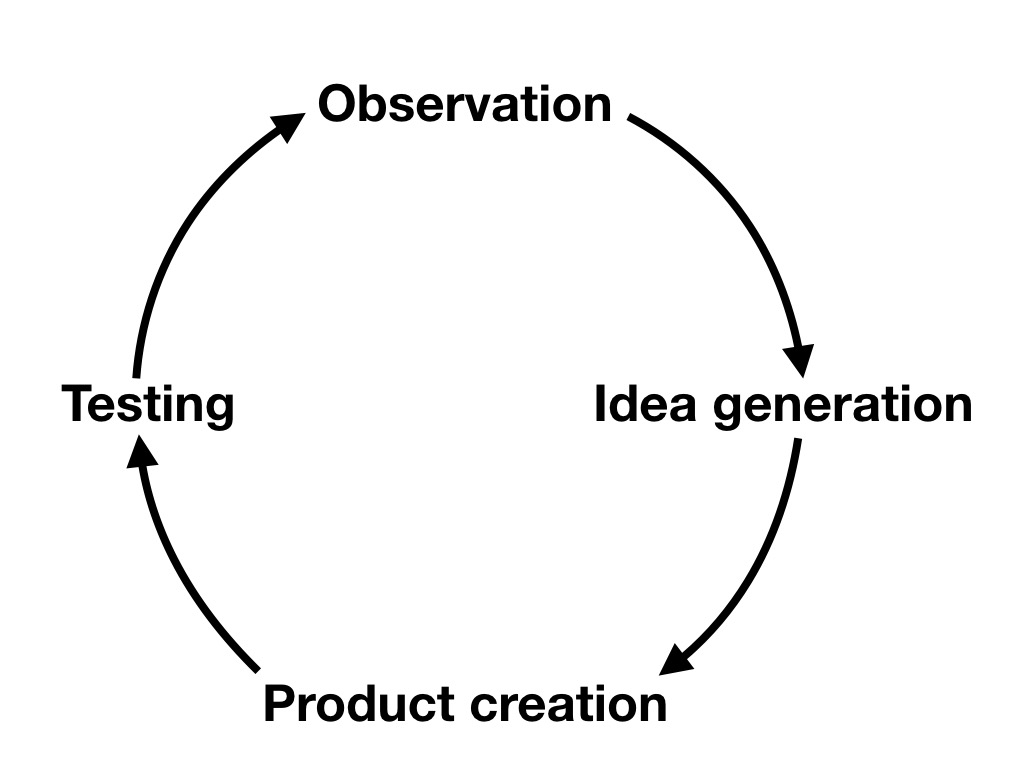
\includegraphics[width=0.5\textwidth]{ProductCreation}
\caption{Redogörelse för de fyra stegen i designprocessen vid användning av Kibana
.}
\end{figure}

 \begin{tabular}{|p{3cm}|p{3cm}|p{3cm}|p{3cm}|}
      \hline
     \textbf{Designkrav} & \textbf{Lösningar} & \textbf{Visualisering} & \textbf{Fält}\\
     \hline
  \multirow{3}{3cm}{Hur många bilar åker igenom varje betalstation och/ eller stad?} &  Trafikintensitet baserad på stad & Taggmoln  & SkatteObjekt\\\cline{2-4}
  & \multirow{2}{3cm}{Trafikintensitet baserad på betalstationer} & Karta med koordinater
& Geografisk Placering\\\cline{3-4}  
  & &  Taggmoln
& Betalstationer \\ \hline


  \multirow{2}{3cm}{Varifrån kommer bilar som åker genom betalstationerna?} &  Kommun där fordonsägare bor & Karta med geografiska områden  & Kommun\\\cline{2-4}
  &Län där fordonsägare bor
 & Karta med geografiska områden  & Län\\ \hline
 
Hur många fordon som passerade den senaste minuten? &Antal fordon
 & Antal  & PassageObjekt\\ \hline
 
 \multirow{2}{3cm}{Hur ser trafikfördelningen ut baserad på riktning?} &  Riktnings-fördelning&Cirkeldiagram& Riktning\\\cline{2-4}
  &Körfälts-fördelning 
 & Cirkeldiagram  & Körfält\\ \hline
 
 \multirow{2}{3cm}{Vilken är den mest populära fordonstypen?} &  Trafikintensitet baserad på fordonstyp & Cirkeldiagram& Fordonstyp\\\cline{2-4}
  &Trafikintensitet baserad på fordonstyp för de mest populära betalstationerna 
 & Stapeldiagram  & TidsStämpel, Betalstation, Fordonstyp\\ \hline


\end{tabular}


\chapter{Analys och diskussion}
Analys och diskussion
\blindtext


\chapter{Slutsatser}
Slutsatser
\blindtext

\chapter{Källförteckning}
Källförteckningen.


\chapter{Bilagor}


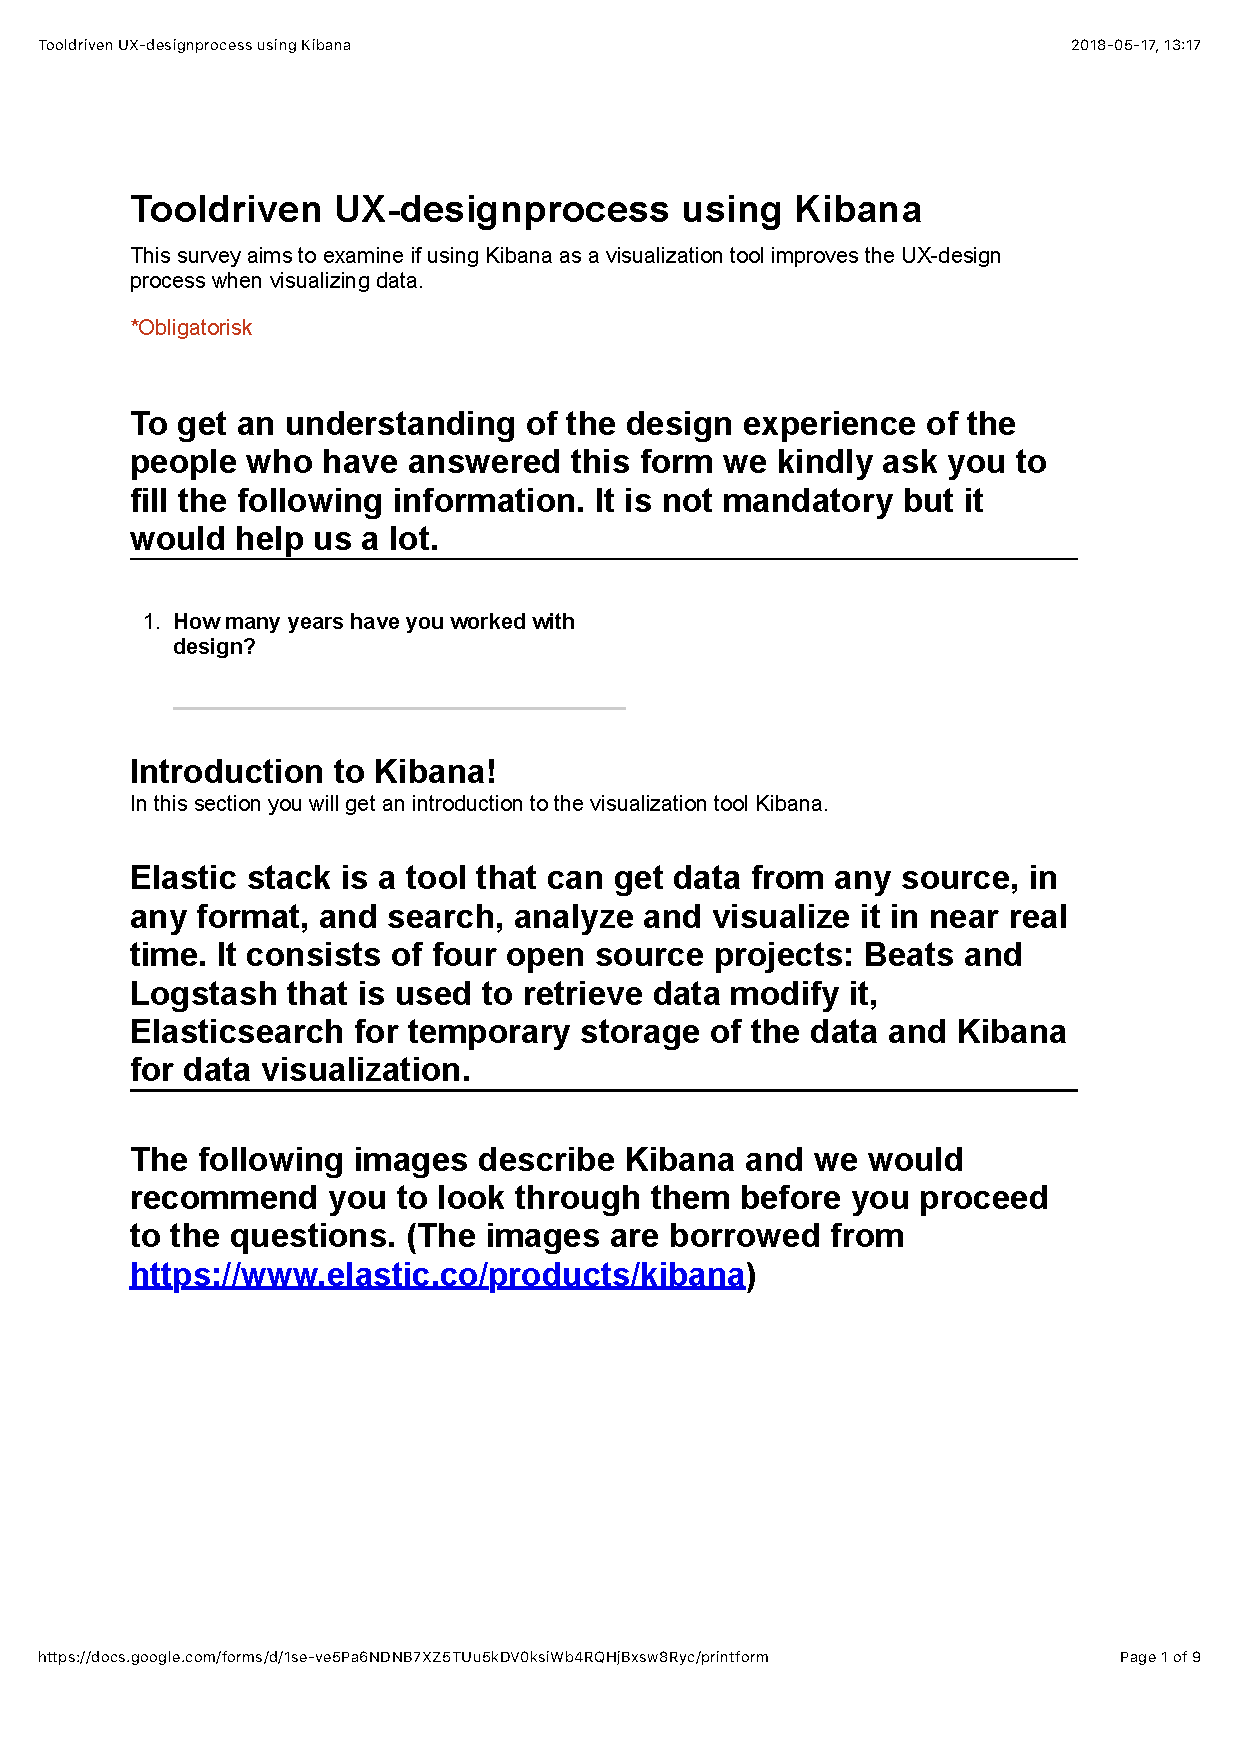
\includepdf[pages={-}]{UX_designprocess.pdf}


\end{document}
